\documentclass[../main/main.tex]{subfiles}

\newdate{date}{16}{11}{2020}

% \begin{figure}[h!]
% \centering
% \includegraphics[page=6,width=0.8\textwidth]{../lessons/pdf_file/17_lecture.pdf}
% \end{figure}

%\displaydate{date}. Compiled:  \today. Alice.

\begin{document}

\pagestyle{plain}

\section{Lecture 17}


\subsubsection*{Slide 1}

\begin{minipage}[]{0.5\linewidth}
\centering
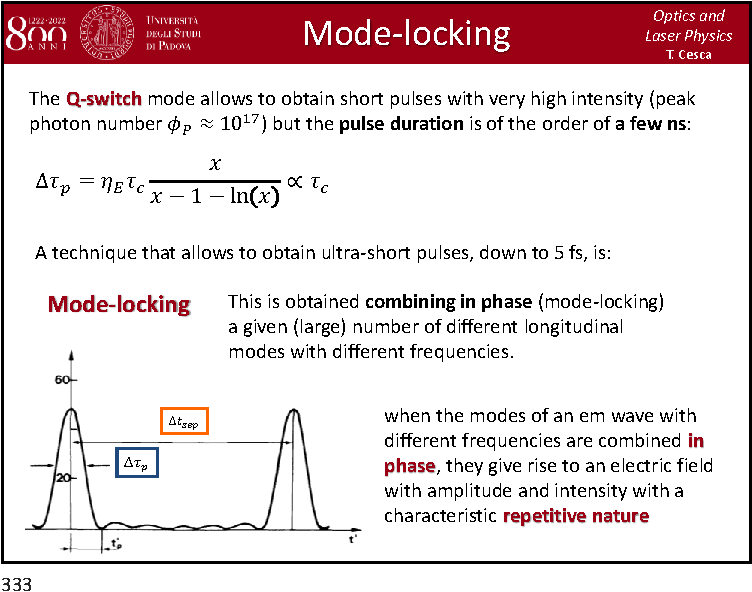
\includegraphics[page=1,width=1\textwidth]{../lessons/pdf_file/17_lecture.pdf}
\end{minipage}
\hspace{0.3cm}\vspace{0.3cm}
\begin{minipage}[c]{0.47\linewidth}

Is there a technique to obtain ultra-short pulses of the order of fs? It is \textbf{mode-locking}.

The basic idea is to lock \textbf{in phase} a large number of longitudinal modes. We obtain pulses with a given pulse duration and with a temporal separation.

\end{minipage}

\subsubsection*{Slide 2}

\begin{minipage}[]{0.5\linewidth}
\centering
\includegraphics[page=2,width=1\textwidth]{../lessons/pdf_file/17_lecture.pdf}
\end{minipage}
\hspace{0.3cm}\vspace{0.3cm}
\begin{minipage}[c]{0.47\linewidth}

It is different if we combine modes with random phases. We do not obtain a repetive nature of the electric field but spice as shown here.

Instead, for mode-locking we combine in phase the modes. We will see that the larger is the number of the modes, the shorter is the pulse duration that we can obtain.

\end{minipage}

\subsubsection*{Slide 3}

\begin{minipage}[]{0.5\linewidth}
\centering
\includegraphics[page=3,width=1\textwidth]{../lessons/pdf_file/17_lecture.pdf}
\end{minipage}
\hspace{0.3cm}\vspace{0.3cm}
\begin{minipage}[c]{0.47\linewidth}

Let us consider to have different \textbf{longitudinal modes} oscillating in the cavity and with a frequency separation \( \Delta \nu _{sep} \).

If we do not do anything we have several longitudinal mode with a bandwidth which is the bandwidth of the gain of the medium.

\( E(t) \) is the electric field amplitude of the m-th mode. Let us assume to simplify the problem and suppose we are able to have \( N \) modes with the same amplitude and oscillating at the same time in the laser cavity.

The total amplitude of the electric field in the cavity is given by the sum of all these nodes.

The difference in terms of angular frequency is \( 2 \pi \Delta \nu _{sep} \).

\end{minipage}

\newpage

\subsubsection*{Slide 4}

\begin{minipage}[]{0.5\linewidth}
\centering
\includegraphics[page=4,width=1\textwidth]{../lessons/pdf_file/17_lecture.pdf}
\end{minipage}
\hspace{0.3cm}\vspace{0.3cm}
\begin{minipage}[c]{0.47\linewidth}

If these modes oscillates with \textbf{random phases} and if the number of nodes is sufficiently large, when we calculate the intensity we obtain that it is proportional to \( N I_0 \).

If the modes oscillates in \textbf{phase} (so if we mode lock the modes). We assume that all the phases for each \( m \) we have \( \Phi _0 \).

\end{minipage}

\subsubsection*{Slide 5}

\begin{minipage}[]{0.5\linewidth}
\centering
\includegraphics[page=5,width=1\textwidth]{../lessons/pdf_file/17_lecture.pdf}
\end{minipage}
\hspace{0.3cm}\vspace{0.3cm}
\begin{minipage}[c]{0.47\linewidth}

The intensity is given now by this expression which reminds the equations which describe interference. Since the modes are locked in phase, we are having them interfering contructively. We obtain a figure of interference in the time domain!

\end{minipage}

\subsubsection*{Slide 6}

\begin{minipage}[]{0.5\linewidth}
\centering
\includegraphics[page=6,width=1\textwidth]{../lessons/pdf_file/17_lecture.pdf}
\end{minipage}
\hspace{0.3cm}\vspace{0.3cm}
\begin{minipage}[c]{0.47\linewidth}

Let us see how to calculate the most relevant parameter.

To calculate \( \Delta t_{sep} \), we need to calculate at which time we get a maximum: when the denominator goes to zero.

The intensity of the peak is proportional to \( N^2 \), the square value of the number of modes you are locking in phase.

\end{minipage}

\newpage

\subsubsection*{Slide 7}

\begin{minipage}[]{0.5\linewidth}
\centering
\includegraphics[page=7,width=1\textwidth]{../lessons/pdf_file/17_lecture.pdf}
\end{minipage}
\hspace{0.3cm}\vspace{0.3cm}
\begin{minipage}[c]{0.47\linewidth}

To calculate the temporal duration \( \Delta \tau _p \), we compute the difference in time between the position of two minima around one maximum.

\( N \Delta \nu _{sep} \) is equal to the \( \Delta \nu _0 \), which is the \textbf{gain bandwidth} (since you obtain gain only for the nodes in the gain bandwidth).

The larger is the gain bandwidth, the shorter is the pulse duration. So, to realize ultra fast pulses you need to work with active media with large bandwidth.

\end{minipage}

\subsubsection*{Slide 8}

\begin{minipage}[]{0.5\linewidth}
\centering
\includegraphics[page=8,width=1\textwidth]{../lessons/pdf_file/17_lecture.pdf}
\end{minipage}
\hspace{0.3cm}\vspace{0.3cm}
\begin{minipage}[c]{0.47\linewidth}

Nd:glass has a much larger bandwidth than in Nd:YAG!

\end{minipage}

\subsubsection*{Slide 9}

\begin{minipage}[]{0.5\linewidth}
\centering
\includegraphics[page=9,width=1\textwidth]{../lessons/pdf_file/17_lecture.pdf}
\end{minipage}
\hspace{0.3cm}\vspace{0.3cm}
\begin{minipage}[c]{0.47\linewidth}

It is the typical laser to obtain pulsed operation. It has a very very larg bandwidth!

\end{minipage}

\subsubsection*{Slide 10}

\begin{minipage}[]{0.5\linewidth}
\centering
\includegraphics[page=10,width=1\textwidth]{../lessons/pdf_file/17_lecture.pdf}
\end{minipage}
\hspace{0.3cm}\vspace{0.3cm}
\begin{minipage}[c]{0.47\linewidth}

With He-Ne laser we obtain a much longer pulse duration.

The basic idea of mode-locking is to lock in phase a large number of modes and to have them you have a large bandwidth in our active medium: the larger is the bandwidth the shorter is the pulse duration!

\end{minipage}

\subsubsection*{Slide 11}

\begin{minipage}[]{0.5\linewidth}
\centering
\includegraphics[page=11,width=1\textwidth]{../lessons/pdf_file/17_lecture.pdf}
\end{minipage}
\hspace{0.3cm}\vspace{0.3cm}
\begin{minipage}[c]{0.47\linewidth}

The question now is how it is possible to lock in phase different longitudinal modes experimentally?

We use an \textbf{optical shutter} in the cavity that we are able to control. When the shutter is open, all the electric fields of all the modes will be maximize (opening the shutter means reducing losses in the cavity for all the modes in the cavity) at the same time.

An \textbf{active shutter} is an electro-optic device. It has the drawback to open exactly the shutter each time the pulse arrive in the shutter itself. You have to be very carefull in controlling the moments in which you open the shutter.

A \textbf{passive shutter} is a non-linear optical element. In particular it is a material which is able to work as a \emph{saturable absorber}. It becomes transparent to radiation if the intensity of the beam is larger than the saturation intensity, in particular it has a \textbf{low} saturation intensity!

\end{minipage}

If the pulse is sufficiently intense, it will open the shutter. So, it is the material itself which know when to open.
In particular, \textbf{passive shutters are typically faster than active ones}.

So, we need some noise to trigger the shutter opening.
A spike intensity at the beginning open the shutter. From that time, when a peak arrive it will open the shutter.

(?)

\subsubsection*{Slide 12}

\begin{minipage}[]{0.5\linewidth}
\centering
\includegraphics[page=12,width=1\textwidth]{../lessons/pdf_file/17_lecture.pdf}
\end{minipage}
\hspace{0.3cm}\vspace{0.3cm}
\begin{minipage}[c]{0.47\linewidth}

The position at which you place the shutter is important: you need to have a shutter which opens every time a pulse is arriving on it (independently on active or passive shutter).

If the separation in time is given \( 2L/c \), which correspond to the situation in which a pulse is making a complete pass back and forth within the cavity. This separation means that the shutter has to be placed exactly at the position of one of the two mirrors.
For all the other modes, they will find the shutter close.

It is possible to select other configuration, as for instance with a time separation of \( L/c \). In this case the shutter is in the middle of the cavity.

For an active shutter you need to open the shutter when the pulse arrive.


The last configuration is for a ring cavity for which the position of the shutter is irrelevant! That is why ring csavity are useful.

\end{minipage}

\subsubsection*{Slide 13}

\begin{minipage}[]{0.5\linewidth}
\centering
\includegraphics[page=13,width=1\textwidth]{../lessons/pdf_file/17_lecture.pdf}
\end{minipage}
\hspace{0.3cm}\vspace{0.3cm}
\begin{minipage}[c]{0.47\linewidth}

This is a photon of Nd:YAG mode-locking.

The shutter is at the position of the mirror 1.

There is not only the \textbf{oscillator} part, but also the \textbf{amplifier}.



\end{minipage}

\subsubsection*{Slide 14}

\begin{minipage}[]{0.5\linewidth}
\centering
\includegraphics[page=14,width=1\textwidth]{../lessons/pdf_file/17_lecture.pdf}
\end{minipage}
\hspace{0.3cm}\vspace{0.3cm}
\begin{minipage}[c]{0.47\linewidth}

Hence, in mode-locking we obtain a train of pulses.

\end{minipage}

\subsubsection*{Slide 15}

\begin{minipage}[]{0.5\linewidth}
\centering
\includegraphics[page=15,width=1\textwidth]{../lessons/pdf_file/17_lecture.pdf}
\end{minipage}
\hspace{0.3cm}\vspace{0.3cm}
\begin{minipage}[c]{0.47\linewidth}

It is an example of a ring cavity laser operating in mode-locking. The separation in time is of about 5 ns with a pulse duration of 0.2 ps. The rod is placed at the Brewster angle to minimize the losses in reflection at the edges of the rod.

\end{minipage}

\subsubsection*{Slide 16}

\begin{minipage}[]{0.5\linewidth}
\centering
\includegraphics[page=16,width=1\textwidth]{../lessons/pdf_file/17_lecture.pdf}
\end{minipage}
\hspace{0.3cm}\vspace{0.3cm}
\begin{minipage}[c]{0.47\linewidth}

Let us make an exercise about the mode-locking.

For He-Ne we can assume \( n = 1 \)!

\end{minipage}

\subsubsection*{Slide 17}

\begin{minipage}[]{0.5\linewidth}
\centering
\includegraphics[page=17,width=1\textwidth]{../lessons/pdf_file/17_lecture.pdf}
\includegraphics[page=18,width=1\textwidth]{../lessons/pdf_file/17_lecture.pdf}
\end{minipage}
\hspace{0.3cm}\vspace{0.3cm}
\begin{minipage}[c]{0.47\linewidth}

We can neglect the presence of the cell even it has a larger refractive index wrt the environment because the tickness is very low.



\end{minipage}




\end{document}
